\chapter{Related Work}\label{sec:related-work}

This Chapter covers relevant techniques for data visualization and the related work in this area of research.
After introducing visualization techniques, related work on interaction aspects in \cmvs{} is outlined in Section~\ref{sec:related-work:interaction-theory}

\section{Foundations}\label{sec:related-work:foundations}
This section introduces terminology, describes the development and shows examples of each data visualization technique.
Advantages and disadvantages of certain data visualization are emphasized.

\subsection{Data visualization}
Data visualization is a means of visual communication and have steadily developed since the 16th century~\cite{Friendly2001}.
It is a generic term, expressing all kinds of effort to put data into visual context to help people understand the significance of data~\cite{Rose2017}.
Data visualization today goes beyond standard charts and graphs used in spreadsheet applications and covers also infographics, heat maps, geographic visualizations and tree maps.
Otherwise abstract information is visually represented, making complex data more accessible, understandable and usable.

\textcite{Kusinitz2014} mentions that the human brain processes visual information 60,000 times faster than text and visual content makes up even 93\% of all human communication.
According to the Interaction Design Foundation the purpose of data visualizations is twofold:
Sense-making and communication.

Statistical information is abstract and in data visualization ``we must find a way to give form to that which has none.''~\cite{Few2013}
Successful data visualizations helps the human user to derive knowledge and meta data from the visualization itself.
\textcite{Nocke2002} call this ``visual data mining''.

\subsection{Data-driven \dss{}}
Data-driven \dss{} are applications to support businesses and organizational decision-making activities in which data visualizations play a key part~\cite{Nada2007}~\cite{Poleto2015}.
A common expression by impatient managers who can not afford to wade through lengthy reports has even become the title of a book about \dss{}:
Stephen Few's ``Show me the numbers''.

In the business context, sales managers demand a quick access on the latest data with all relevant visualizations at once.
Examples of this kind of \dss{} are called e.g.\ ``decision cockpit'' or ``business sphere''\cite{Davenport2013}.

We can expect to see these technologies more in more in business applications.
\textcite{McAfee2012} from the MIT Center of Digital Business showed that organizations driven most by data-based decision making had 4\% higher productivity rates and 6\% higher profits.

However, little research has been done regarding the performance of \cmvs{} in the field of decision making.
There might be a great potential.
In 1997 \textcite{Mayer1997} conducted eight studies to compare the effect of using multimedia on university students.
The studies showed that when using combined visual and verbal explanations the generation of creative problem solutions increased by an average of more than 50\%.

Apparently, the application of combined data visualization techniques in decision making is a promising strategy.

\subsection{Visual Variables}\label{sec:related-work:visual-variables}
French cartographer Jaques Bertin introduced seven visual variables in 1967~\cite{Bertin2010}.
We can see an example for each in Figure~\ref{fig:related-work:visual-variables}.
These visual variables are used in cartography but can also be applied to data visualization in general.
\textcite{Carpendale2003} explains in detail their use in computational information instead of printed cartography.
\textcite{Garlandini2009} put these visual variables under systematic validation procedures.
The authors conclude that the variable \attr{size} provides the most accurate and efficient performance while the variable \attr{orientation} provides the least performance.
\begin{figure}[ht]
  \centering
  \includegraphics[width=\textwidth]{figures/related-work/visual-variables.png}
  \caption{Bertin's~\cite{Bertin2010} original visual variables.}\label{fig:related-work:visual-variables}
\end{figure}
Bertin's visual variable play a role in interaction aspects of \cmvs{} as they are used to communicate the effect of an interaction.
A highlighted data point can be highlighted by changing the colour of an area or increasing the size of a point.

\subsection{Treemaps}
The visualization of hierarchical data has a long tradition.
The traditional visual representation of a tree is a directed graph with the root node at the top, as seen in Figure~\ref{fig:related-work:tree-graph}.
\begin{figure}[ht]
	\centering
	\includegraphics[width=\textwidth]{figures/related-work/tree.pdf}
	\caption{Traditional visualization of a tree in form of a directed graph with edges and nodes and the root node at the top}\label{fig:related-work:tree-graph}
\end{figure}
An everyday use case is a directory tree example of a file system.
E.g.\ a file browser or the command line utility \texttt{tree} on UNIX based operating systems.
As \textcite{Shneiderman1992} mentions, this visualization becomes increasingly large when displaying more than one level and soon exceeds the entire screen size.

\textcite{Johnson1991} proposes the tree map visualization technique, in which each node is a rectangle whose area is proportional to a specified dimension.
The hierarchy in tree maps is expressed with tiles instead of nodes and every child node to parent node relation is expressed with a parent tile containing other tiles.

We can see two examples of tree maps in Figures~\ref{fig:related-work:treemap-german-exports-1} and~\ref{fig:related-work:treemap-german-exports-2}.
German exports are divided in generic groups like ``Machines'' and ``Chemical Products'' and include more specific groups like ``Cars'' and ``Packaged Medicaments''.
The user can click on a drop-down menu to change the current level of hierarchy, only leaf nodes are displayed at a time.

The big advantage of tree maps is that they are space-filling visualizations, i.e.\ they make 100\% use of the available screen size.
A tree map will, unlike a graph representation of a tree, never exceed the size of the screen.

The area of the tiles can be mapped to a data attribute, e.g.\ the file size on disk or, in cases of Figures~\ref{fig:related-work:treemap-german-exports-1} and~\ref{fig:related-work:treemap-german-exports-2}, the percentage of export quota.
Thus, a tree map can display even more information than a traditional graph representation.
A disadvantage of tree maps is the variable size of each node.
If more and more nodes are displayed, the size of each tile will get smaller and smaller and there might not be enough space to display a label.
You can see this problem occur in Figure~\ref{fig:related-work:treemap-german-exports-2}.
\begin{figure}[ht]
    \centering
    \copyrightbox[b]{%
        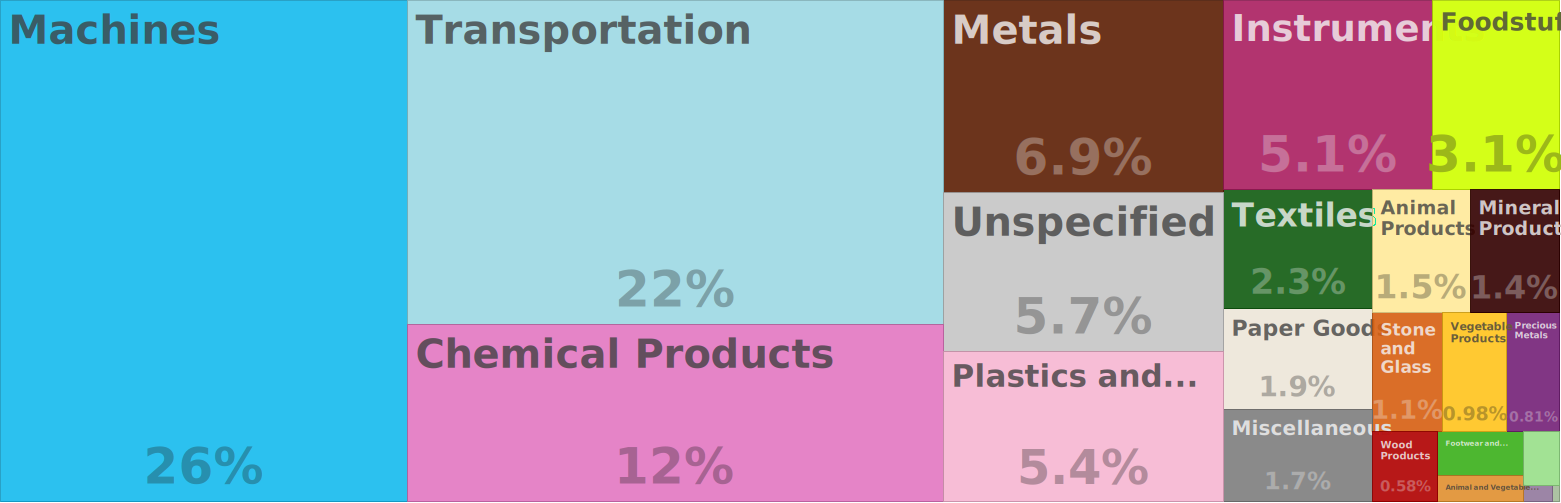
\includegraphics[width=\textwidth]{figures/related-work/en_profile_country_deu.pdf}}{%
        \hfill \ccAttribution{} \ccShareAlike{} Observatory of Economic Complexity~\cite{Macro2017}
    }
    \caption{A two dimensional tree map of Germany's foreign trade quota of exports, showing only the first hierarchy level.}
    \label{fig:related-work:treemap-german-exports-1}
\end{figure}

\begin{figure}[ht]
    \centering
    \copyrightbox[b]{%
        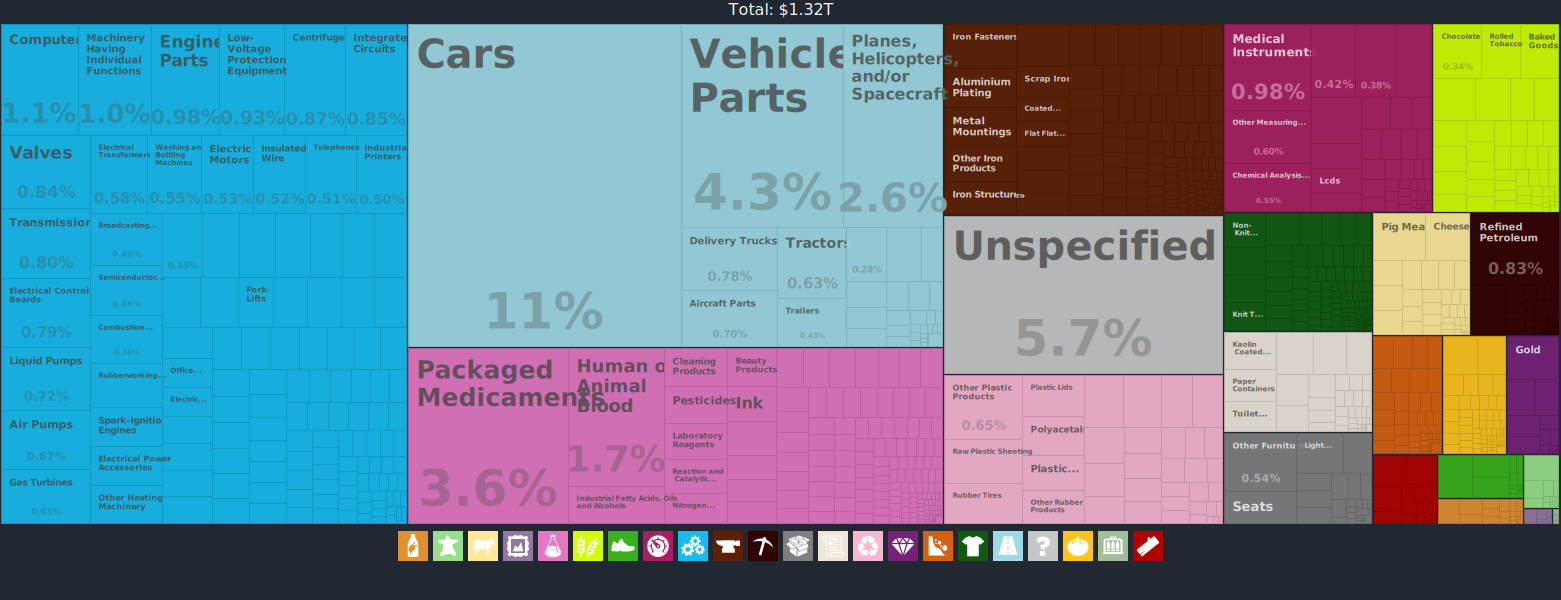
\includegraphics[width=\textwidth]{figures/related-work/en_profile_country_deu_2.pdf}}{%
        \hfill \ccAttribution{} \ccShareAlike{} Observatory of Economic Complexity~\cite{Macro2017}
    }
    \caption{A two dimensional tree map of Germany's foreign trade quota of exports, showing a hierarchy of depth ``HS4''}\label{fig:related-work:treemap-german-exports-2}
\end{figure}
If tree maps are used to visualize geographic data like municipalities, real estates or streets, the placement of nodes depends on the tiling algorithm and not the geographic location on a map.
Let's say a tree map visualizes a hierarchy of federal states and municipalities, the area of each tile mapped to the total population of administrative district.
Even if the membership hierarchy is matched by the tree map, the placement of districts in the same hierarchy level is based on their total population and not their geographic location.

\subsubsection{3D tree maps and \tmaps{}}
3D tree maps is a concept introduced by \textcite{Bladh2004} in 2004.
The authors transfer the concept of tree maps from two dimensional into three dimensional space, transforming tiles to blocks.
They introduce StepTree~\cite{Bladh2004}, which is a three dimensional tree map to display a directory layout of a file system.
It ``differs from Treemap in that it employs three dimensions by stacking each subdirectory on top of its parent directory.''

3D tree maps are superior to 2D tree maps for tasks with a pronounced topological challenge.
User perform significantly better in interpreting the hierarchical structure.
However, 3D visualizations also introduce some disadvantages.
Blocks can superimpose each other, forcing the user to navigate the view point.
The navigation of the view point itself is an increase of complexity not present in two dimensional tree maps.

The term \tmap{} was coined by \textcite{Limberger2016} in 2016.
A \tmap{} is just an ordinary 3D tree map, but it has all blocks attached to the ground, or more specifically, attached to the parent block.
We can see an example of a \tmap{} in figure~\ref{fig:research:ua_treemap}.
The term \tmap{} is used throughout this thesis to emphasize this usually existing constraint.

\begin{figure}[ht]
  \centering
  \copyrightbox[b]{%
    \includegraphics[width=\textwidth]{figures/related-work/2_5D_treemap_example}}{%
    \hfill \textcopyright{} Hasso-Plattner-Institut\cite{Doellner2017}
  }
  \caption{Example of a \tmap{}}\label{fig:research:ua_treemap}
\end{figure}

\subsection{Geovisualization}
The umbrella term ``Geovisualization'' covers visualization techniques for the visual exploration, analysis, synthesis and presentation of geospatial data (any data having geospatial  referencing)~\cite{Maceachren2001}.
The entities of gespatial data may include buildings, streets, landmasses, terrain, administrative districts and also moving entities like cars.
In this section we introduce four types of geographic visualization, which are commonly used to display both geographic and hierarchic data.


\subsubsection{Choropleth maps}
Choropleth maps are thematic maps in which areas are shaded or patterned in proportion to the statistical variable being displayed on the map.
A popular use case is the display of population density or per-capita income.
We can see an example of a choropleth map in Figure~\ref{fig:related-work:choropleth}, showing the percentage of obese population in the US\@.
Choropleth maps are very popular and therefore many people are familiar with them already.
A downside of choropleth maps is that larger regions may appear more emphasized than smaller ones, since the entire area of regions is coloured.
Another disadvantage of choropleth maps is the common error of incorrect encoding:
If they display absolute numbers, e.g.\ total population or proceeds of crime, rather than relative numbers, e.g.\ population density of unemployment rate.

\begin{figure}[ht]
  \centering
  \copyrightbox[b]{%
    \includegraphics[width=\textwidth]{figures/related-work/choropleth}}{%
    \hfill National Center for Chronic Disease Prevention and Health Promotion~\cite{NCCDPHP2017}
  }
  \caption{%
    Choropleth Map of Obesity in the United States in 2008.
    Present of population classified as ``obese'' (Body Mass Index in excess of 30), by state.
  }\label{fig:related-work:choropleth}
\end{figure}

\subsubsection{Other thematic maps}

There is a variety of geographic visualizations similar to choropleth maps.
Some of those have advantages compared to choropleth maps or enable to visualize other kinds of data.

\textbf{Flow maps} is a graph visualization of regions and their relationships.
You can see a flow map in Section~\ref{sec:analysis:examples:single} in Figure~\ref{fig:analysis:geographical}.
Flow maps place stroked lines on top of a geographic map to connect two geographic entities.
These connections can encode more data attributes in the size or the colour of the stroke, its direction or shape.
They often display the flow of goods or the migration of people.


\textbf{Graduated Symbol or Proportional Symbol Maps} place a symbol on each region of the map, the symbol representing one or more data attributes.
These maps are a good alternative to choropleth maps as they overcome the disadvantage of emphasizing larger areas.
As \textcite{Heer2010} point out, these symbols can visualize many more data attributes, e.g.\  by symbol size, shape and colour.

\textbf{Cartograms} encode a data attribute in the size of an area.
For this reason geographic regions in cartograms appear distorted.
A common example is to redraw the size of a country based on the population or gross domestic product of a country.
Area cartograms may be contiguous or noncontiguous, depending on the applied layout algorithm.

This work uses a choropleth map for the geographic visualization because of its widespread recognition.

\subsection{Coordinated Multiple Views}
\cmvs{} are a combination of data visualizations of the same data set in multiple views, often side-by-side.
According to \textcite{Roberts2007} \cmvs{} is just ``a specific exploratory visualization technique that enables users to explore their data''.
Because ``the overall premise for the technique is that users understand their data better if they interact with the presented information and view it through different representations.''~\cite{Roberts2007}

We can see an example of a \cmv{} in Figure~\ref{fig:related-work:cmv}
It displays spatial and temporal attributes of pictures in a picture database, as well as continuous attributes like popularity and number of comments.
\begin{figure}[h]
  \centering
  \copyrightbox[b]{\includegraphics[width=\textwidth]{figures/related-work/cmv}}{\hfill Dukevis\cite{Dukevis2017}}
  \caption{\cmv{} displaying the popularity, number of comments, location and time of pictures in a picture data base}\label{fig:research:cmv}
\end{figure}
The user can move the mouse cursor over each item in the scatter plot and the graduated symbol map and the corresponding item is highlighted with a larger stroke in all other views.
On the time line below, the user can also filter for pictures in a certain time frame by dragging the mouse from lower to upper limit.

\begin{figure}[h]
  \centering
  \copyrightbox[b]{\includegraphics[width=\textwidth]{figures/related-work/brushing_linking}}{\hfill Crossfilter\cite{Bostock2017}}
  \caption{Airline on-time performance: Correlation of time of day with arrival delay. Most recent flight with a delay of more than 100 minutes selected.}\label{fig:research:brushing-linking}
\end{figure}

\subsubsection{Brushing and Linking}
Brushing and linking is a common interaction pattern found in \cmvs{} and often a crucial part of these visualization.
``The technique of brushing is the principle approach, where elements are selected (and highlighted) in one display, concurrently the same information in any other linked display is also highlighted.''\cite{Roberts2007}

We can see an example in Figure~\ref{fig:research:brushing-linking}.
It displays an on-time performance of airlines, visualized with the ``Crossfilter'' javascript library.

This library is also one of the very few examples of an interaction framework for \cmvs{}.
However, this library is unmaintained as of December 2017, the most recent commit dating back to March 2016.

Each of the flight in the data set has an hour and a date for departure, a arrival delay, which can also be negative, and a traveled distance in miles.
The user can ``brush'' the data by selecting an interval by dragging the mouse.
The respective view will become a primary view and display the deselected items with a grey colour.

All other views become secondary views and display only selected items.
The visualization takes the most recent 80 flights from the database that match all given filters.
The user can further filter for items by dragging another interval in one of the secondary views.

This technique of propagating interactions to other views is called ``linking''.

Figure~\ref{fig:research:brushing-linking} shows a filter for travels with a long delay, i.e.\ from 120 minutes to the maximum value, see the selection in the upper center.
In the view in the upper left corner in Figure~\ref{fig:research:brushing-linking}, we can see a correlation of long delays with the time of the day.

\section{Libraries, Frameworks and Standards}

\textbf{TypeScript}
TypeScript is a typed superset of JavaScript that compiles to plain JavaScript.
It provides optional static typing, classes and interfaces.


\textbf{PubSubJS} is a topic-based publish/subscribe library written in JavaScript~\cite{PubSubJS2017}.
Topics can be registered hierarchically, with subtopics delimited by dots.
A subscription to topic \attr{mcv.select.focus} will be notified only for \attr{focus} interactions whereas a subscription of \attr{mcv.select} will be notified for both \attr{focus} and \attr{highlight} interactions.
Furthermore, topics are published asynchronously, so if the user interacts with a visualization, that does not block code execution.

\textbf{GeoJSON}
GeoJSON is a format for encoding a variety of geographic data structures~\cite{GeoJSON2017}.
Based on JSON, it can simple geographic features like points, lines and areas and reserves a properties object for non-spatial attributes.

\textbf{Leaflet}
Leaflet is the leading open-source JavaScript library for mobile-friendly interactive maps~\cite{Leaflet2017}.
It has support for GeoJSON which makes it very easy to display tiled web maps with interactive overlays.

\textbf{ReactJS}
ReactJS is an open-source JavaScript library to build user interfaces and allows to create reusable UI components.
React renders HTML on the client, it changes the page without reloading the page.
The framework corresponds with the View in the Model-View-Controller pattern.
React components are structured hierarchically, with each component having dedicated responsibility.


\section{Interaction Theory}\label{sec:related-work:interaction-theory}
According to \textcite{Ho2013} interactions are a crucial part of data visualizations, yet most research in the area of data visualization still focuses on visual representations.
Roughly speaking, research on interaction falls into these groups:
How to categorize interaction techniques?
How to find new interaction techniques and apply those to visualizations?

\todo[inline]{Give a rough overview of this section}
\subsection{Interaction Categories}\label{sec:related-work:interaction-theory:categories}
\textcite{Shneiderman1996} classifies interactions into these groups:
\begin{enumerate*}[label=(\arabic*)]
  \item
    Gain an \emph{overview} of the entire collection,
  \item
    \emph{zoom} in on items of interest,
  \item
    select an item or group and get \emph{details} when needed,
  \item
    view \emph{relationships} among items,
  \item
    keep a \emph{history} of actions to support undo,
  \item
    allow \emph{extraction} of sub-collections and of the query parameters.
\end{enumerate*}

In 1997 \textcite{Shneiderman1996} classified interactions into these groups:
\begin{enumerate*}[label=(\arabic*)]
  \item
    Gain an \emph{overview} of the entire collection,
  \item
    \emph{zoom} in on items of interest,
  \item
    select an item or group and get \emph{details} when needed,
  \item
    view \emph{relationships} among items,
  \item
    keep a \emph{history} of actions to support undo,
  \item
    allow \emph{extraction} of sub-collections and of the query parameters.
\end{enumerate*}

Two years later, \textcite{Dix1998} identified these categories:
\begin{enumerate*}[label=(\arabic*)]
  \item
    \emph{Highlight and focus} particular subsets of the data,
  \item
    instead of displaying everything simultaneously \emph{access extra information} by drilling down the data,
  \item
    zoom in and out to give an \emph{overview and context},
  \item
    \emph{change parameters} of the \emph{same representation}, e.g.\ another baseline of a stacked bar char,
  \item
    \emph{change representation} of the \emph{same data} by switching the chart type,
  \item
    \emph{link representations} to determine the relationship between items.
\end{enumerate*}

In 2002, \textcite{Keim2002} comes up with the following classification:
\begin{enumerate*}[label=(\arabic*)]
  \item
    Dynamic \emph{projection} to show all combination of data attributes mapped to the axis of a diagram,
  \item
    focus on a smaller subsets by \emph{filtering} out parts of the data,
  \item
    \emph{zoom} into a subset of the data and get a higher level of detail,
  \item
    preserve an overview of the data during drill-down operations is called \emph{distortion}
  \item
    and finally \emph{link and brush} visualizations, to highlight the same data points in multiple visualizations.
\end{enumerate*}

The most recent classification was done in 2007 by \textcite{Yi2007} listing seven categories:
\begin{enumerate*}[label=(\arabic*)]
  \item
    \emph{Select} to mark something as interesting,
  \item
    \emph{explore} to show something else,
  \item
    \emph{reconfigure} to show a different arrangement,
  \item
    \emph{encode} to show a different representation,
  \item
    \emph{abstract/elaborate} show more or less detail,
  \item
    \emph{filter} show something conditionally,
  \item
    \emph{connect} show related items.
\end{enumerate*}

\todo[inline]{The classifications are all redundant! Explain why and choose one classification for later use}
\todo[inline]{Give one example for each category of the chosen classification}

\subsection{Interaction Models}
\todo[inline]{no section without text}

\textbf{Space-Time Cube Operations}
is a concept introduced in 2014 by \textcite{Bach2014} to map temporal data into two dimensional visualizations.
Space-time-cubes are used to model two attributes of continuous data with temporal data along a third axis, therefore the name \emph{cube}.
While the transformations are rather static it is also possible to introduce activity into the transformations.
The authors describe user-independent \emph{animations} and user-controlled \emph{interactions}.
E.g.\ a transformation may display a given slice of the cube.
An animation would display one slice at a time and display the next slice every second.
Whereas the interaction would show the slice determined by a user-controlled slider.
Various transformations and their best use in practice are evaluated in this work.
The work focuses on temporal data and otherwise continuous data.
Interactions are not seen as an abstract entity, that need to be agnostic of the underlying data structure and visualization.
The authors admit ``our framework does not provide much guidance for interaction design: the design space for interactive operations has only been partially explored.''\cite[Other limitations, p.~15]{Bach2014}

\textbf{ITlib\cite{Figueroa2001}} is an architecture and a framework of interaction techniques for virtual reality applications, designed to be extensible and flexible.
New interaction techniques can easily be added and application specific code is seamlessly integrated.
On a low level an interaction technique ``is modeled as a set of filters connected in a small data flow''\cite[Basic concept, p.~2]{Figueroa2001}.
These filters are the smallest process unit in the data flow.
Composed of input and output ports, they communicate with other filters, to receive data input from predecessors and send data output to successors.
The framework specifies and stores the interaction techniques along with its filters, the execution model and the scene in XML documents.
The authors chose XML because it can be parsed easily and they generate code in order to target various virtual reality toolkits and environments.

Even though the system describes interactions in an abstract way, the domain of the framework is clearly the interaction of a human body within a 3D virtual reality.
Certain assumptions are made, including the data model, which is the 3D scene, and human computer interaction devices, like the user's hand or the user's head.
The goal is not to better understand the data, as the data model in this case is the 3D scene, and not statistical data.
Most important, the framework describes interaction techniques for a single viewpoint but not for coordinated multiple views.

\textbf{Focus+Context Visualization} by \textcite{Bjork1999} is one of the few formalizations of information visualizations.
The authors describe this formalization based on first-level and second-level visualization:
\subparagraph{Visualizations} referred to as $IV$, are triples of a set $[D]$ of underlying data, a visual representation $V$ and $I$ which is the possible interaction or manipulation.
\begin{equation}
  IV([D], V, I)
\end{equation}
If $I$ affects $[D]$ we can manipulate the underlying data set.
Examples would be changes in a spreadsheet editor, or a change of the start and end date of an appointment in a calendar.
When $V$ is affected by $I$ the user can manipulate $IV$ in order to change the way $[D]$ is represented, e.g.\ choosing a different level of detail as shown in Figures~\ref{fig:related-work:treemap-german-exports-1} and~\ref{fig:related-work:treemap-german-exports-2}.

\subparagraph{Second-level Visualizations} are information visualizations consecutively applied.
The underlying data set $[D]$ of the previous formula is replaced with some information visualization $IV$, which is compatible with $IV'$.
\begin{equation}
  IV'(IV, V', I')
\end{equation}


Focus+context visualizations are second-level visualizations.
An example given by the authors is the  ``rubbersheet'' visualization, that visually distorts a first-level visualization similar to a magnifier.

